\documentclass[12pt,a4paper]{article}
\usepackage[top=25.4mm, bottom=25.4mm, left=19.1mm, right=19.1mm]{geometry}


\usepackage[latin2]{inputenc}
\usepackage{graphicx}
\graphicspath{ {./images/} }
\usepackage{ulem}
\usepackage{enumitem}
\usepackage{amsmath}
\usepackage[document]{ragged2e}

\setlength{\parindent}{4em}
\setlength{\parskip}{1em}
\usepackage{hyperref}

\usepackage{fancyhdr}
\pagestyle{fancy}
\fancyhf{}
\fancyhead[LO]{\textbf{\small IoT and Smart Analytics}\\
\text{\small A Program by IIITH and TalentSprint}}

\usepackage{xcolor}
\usepackage{lipsum}

\rhead{\begin{picture}(0,0) \put(-250,-2){
\includegraphics[width=9cm]{EXP_06_Images/ts-iisc-logo-pr.png}} \end{picture}}
\cfoot{\thepage}


\begin{document}

\begin{center}
\textbf{\large \\EXPERIMENT 26 }\\[6pt]
Exploring AWS-IoT core: Part-I
\end{center}

\textbf{\large LEARNING OBJECTIVES:}\\[3pt]
At the end of this experiment, participants will be able to:\vspace{-6mm}\begin{enumerate}
 \setlength\itemsep{-0.3em}
\item Create an AWS Account
\item Connect  ESP32 with AWS IoT Core and  test the published data on the MQTT test client 
\item Store the data sent by ESP32 on DynamoDB 

\end{enumerate}

\textbf{\large APPARATUS REQUIRED:}\\
\vspace{-3mm}
\begin{enumerate}
 \setlength\itemsep{-0.3em}
\item ESP32-1-pcs 
\item USB cable-1pcs
\item Breadboard-2pcs
\item Internet Connection 

\end{enumerate}

\begin{justify}
\textbf{\large THEORY}\\[3pt]
Figure1. below shows a generic data flow architecture involving data ingestion to analytics in  AWS IoT. After getting data in AWS IoT core it can be further used in different services. .

\begin{center} 
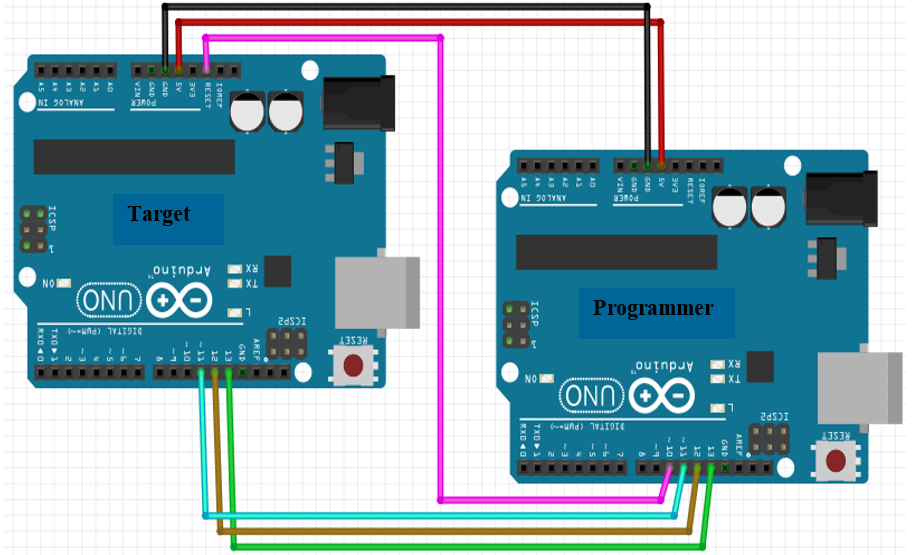
\includegraphics[scale=0.6]{EXP_26_I_Images/fig1.png}
\end{center}
\vspace{-10mm}
\begin{center} {Figure 1.Architecture diagram of data flow}\end{center}

\noindent The steps may differ slightly based on requirements and there are multiple ways of doing the same thing. In the first part of this experiment, we are going to connect the ESP32 to the AWS IoT core and store the data published from the ESP32 into a table in DynamoDB.The diagram below shows the simplest way of creating necessary components in AWS IoT that we are going to follow. Details for each step are given in the procedure.

\begin{center} 
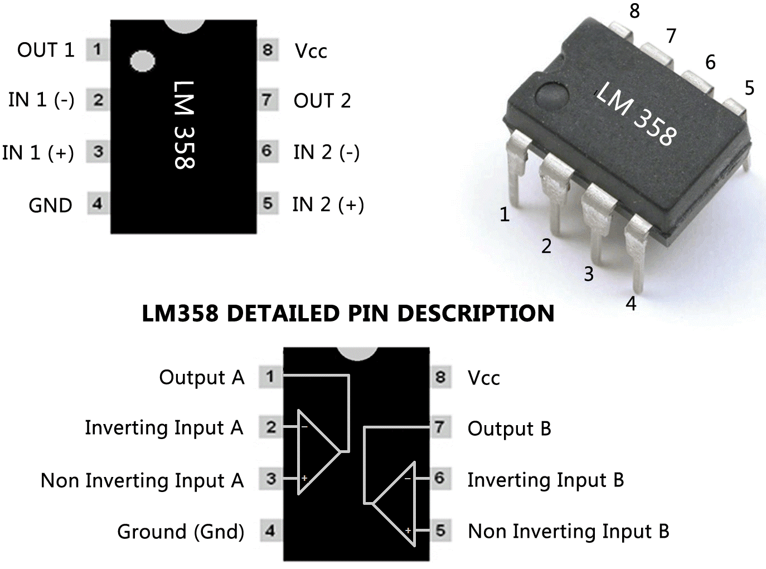
\includegraphics[scale=0.5]{EXP_26_I_Images/fig2.png}
\end{center}
\vspace{-10mm}
\begin{center} {Figure 2.Components in AWS IoT}\end{center}


\noindent \textbf{\large PROCEDURE}\\[6pt]
\textbf{A) Creating an AWS account \& going to AWS IoT core}\\[3pt]
Follow the document named "Creating an AWS account" for account creation and login. After login search  'IoT core' and click on it. A page similar to fig.3 will appear.
\vspace{-5mm}
\begin{center} 
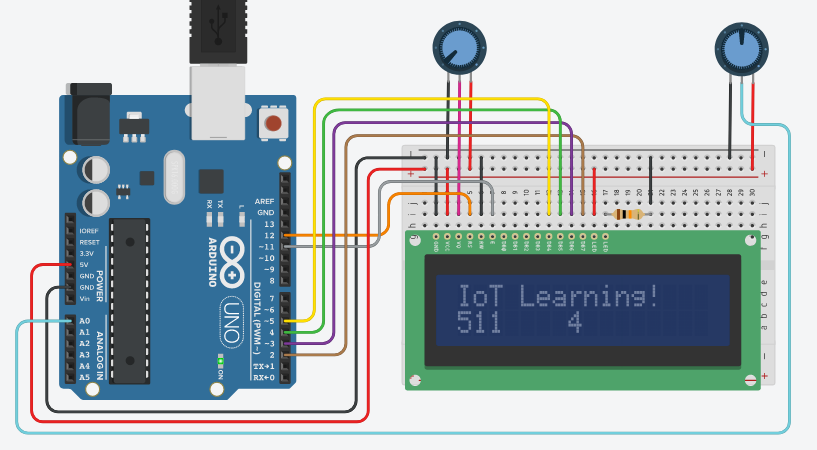
\includegraphics[scale=0.6]{EXP_26_I_Images/fig3.png}
\end{center}
\vspace{-10mm}
\begin{center} {Figure 3.AWS IoT  page}\end{center}
\vspace{3cm}

\textbf{B)	Creating a Thing in AWS IoT}
\vspace{-3mm}
\begin{itemize}
 \setlength\itemsep{-0.3em}
\item Click on \textcolor{blue}{ Manage} $ \rightarrow $ Click on \textcolor{blue}{Things} $ \rightarrow $ Click on \textcolor{blue}{Create things} $ \rightarrow $ Select {Create single thing} $ \rightarrow $ click on Next $ \rightarrow $ Provide \textbf{Thing} name, say esp32 in Things properties $\rightarrow $ Select\textcolor{blue}{ No shadow} $ \rightarrow $ Click on \textcolor{blue}{Next}
\item We can skip the \textbf{Device certificate} part for time being. We will do it later, so choose \textbf{Skip creating a certificate at this time} and click on $ \rightarrow $ \textcolor{blue}{Next}.
\item A Thing having the name \textbf{"esp32"} will be seen as given in fig. 4 below. Click on $ \rightarrow $ \textcolor{blue}{esp32} and notice \textbf{ARN} (Amazon resource number). It will be used later.

\begin{center} 
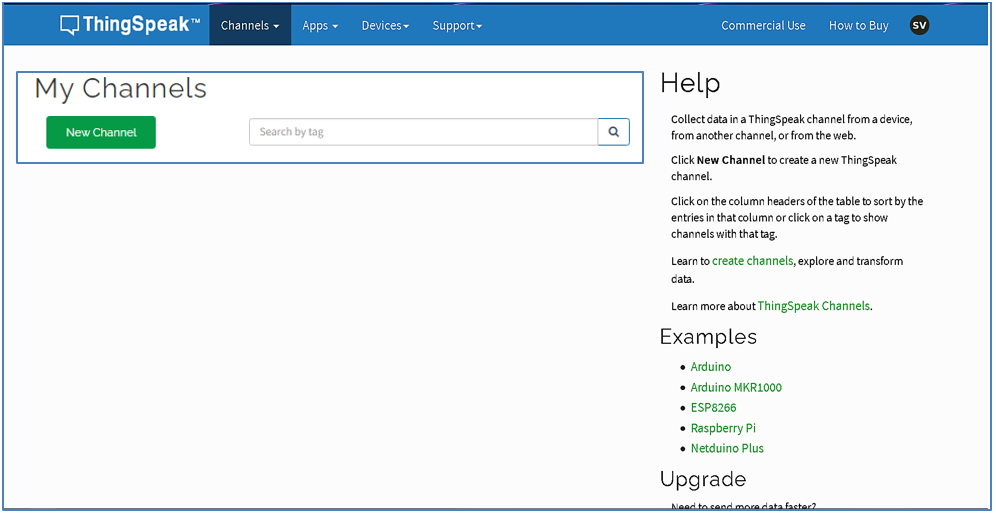
\includegraphics[scale=0.55]{EXP_26_I_Images/fig4.png}
\end{center}
\vspace{-10mm}
\begin{center} {Figure 4.Thing created }\end{center}
\end{itemize}



\textbf{C) Creating certificates and attaching the Thing to them:}
\vspace{-3mm}
\begin{itemize}
 \setlength\itemsep{-0.3em}
\item Click on  \textcolor{blue}{Secure} $ \rightarrow $ Click on \textcolor{blue}{Certificates} $ \rightarrow $ Click on \textcolor{blue}{Create certificates} $ \rightarrow $ Select \textcolor{blue}{Auto-generate new certificate} and select \textcolor{blue}{Active} $ \rightarrow $ Click on Create. A page as given in fig. 5 below will display. Download \textbf{Device certificate, Public key file, Private key file, and Root CA1}  and store all these in a  folder named credentials in your Laptop/PC. 

    \item After downloading $ \rightarrow $ Click on \textcolor{blue}{Continue}. A page with a Certificate ID will display. \textcolor{blue}{Tick on} $ \rightarrow $ small square box in front of Certificate ID and $ \rightarrow $ Click on \textcolor{blue}{Action} $ \rightarrow $ Click on $ \rightarrow $ \textcolor{blue}{Attach a thing} $ \rightarrow $ Choose the thing name that we have created, here \textbf{'esp32'}  $ \rightarrow $ Click on \textcolor{blue}{Attach to thing}.


\begin{center} 
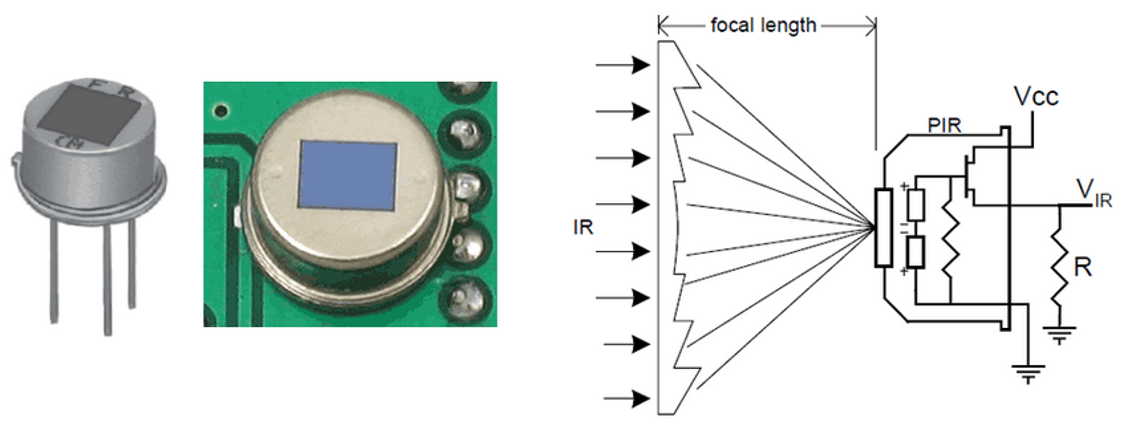
\includegraphics[scale=1]{EXP_26_I_Images/fig5.png}
\end{center}
\vspace{-10mm}
\begin{center} {Figure 5.Certificates Download pages}\end{center}
\end{itemize}


\textbf{D)	Creating Policy and attaching it to the certificate:}
\vspace{-3mm}
\begin{itemize}
 \setlength\itemsep{-0.3em}
\item  	Go to \textcolor{blue}{Secure} $ \rightarrow $ Click on \textcolor{blue}{Policies} $ \rightarrow $ Click on Create policy $ \rightarrow $ Provide \textbf{esp32policy} as \textbf{Policy name} in \textbf{Policy properties}. 

\item Now in \textbf{Policy document} region $ \rightarrow $ Select \textcolor{blue}{Allow} in \textbf{Policy effect} box. Select $ \rightarrow $ *  in the \textbf{Policy action} box. Put $ \rightarrow $  * in the \textbf{Policy resource} box. Click on $ \rightarrow $ \textcolor{blue}{Create}.

\item A policy named \textbf{esp32policy} will be displayed. Now we have to attach a certificate for this policy. Click on $ \rightarrow $ \textcolor{blue}{Certificate} $ \rightarrow $ \textcolor{blue}{Tick on} $ \rightarrow $ small square box in front of Certificate ID and$ \rightarrow $ Click on \textcolor{blue}{Action} $ \rightarrow $ Click on $ \rightarrow $  \textcolor{blue}{Attach apolicy} $ \rightarrow $  Choose the policy name that we have created, here \textbf{'esp32policy'} $ \rightarrow $ Click on \textcolor{blue}{Attach to policies}.
.
\end{itemize}

\vspace{3cm}

\textbf{E) Connecting  ESP32 with AWS IoT Core \& testing with MQTT test client }
\vspace{-3mm}
\begin{itemize}
 \setlength\itemsep{-0.3em}
\item Open the 'AWS\_IoT\_PubSub.ino' script in Arduino IDE and upload in ESP32 after  changing the following parameters:

    \begin{enumerate}
     \setlength\itemsep{-0.3em}
    \item WiFi credential
    \item AWS Endpoint. Go to the $ \rightarrow $ \textcolor{blue}{Settings} and copy the \textbf{Endpoint}. It remains fixed for your account.
    \item Device certificate (xxxxxxxxxx-certificate.pem.crt), Private key (xxxxxxxxx-private.pem.key), Root CA (RootCA1.pem). 
    
    In \textbf{step C)}, we have downloaded all these files. Open these files with Notepad and copy as it is and keep inside the parenthesis of $ \rightarrow $ \textbf{R"KEY( )KEY"}.
    
    \item PUBLISH\_TOPIC, SUBSCRIBE\_TOPIC  can be changed but keep as it is for time being. In THING\_NAME put the name of the Thing that we created in AWS IoT (\textbf{esp32}).\\[3pt]
    \end{enumerate}
\vspace{-3mm}
\item After uploading the script in ESP32, go to the \textcolor{blue}{AWS IoT} $ \rightarrow $ \textcolor{blue}{Test} $ \rightarrow $ \textcolor{blue}{MQTT test Client}, a page as in fig. 6 below will appear. Choose the ' \textcolor{blue}{Subscribe to a topic}' and fill publish topic taking from the Arduino script in the \textbf{Enter the topic filter} box i.e. \textbf{outTopic}. \textbf{Click on} $ \rightarrow $ \textbf{Subscribe}. You can see the payload being received in the box below the topic header as shown in fig. 7.

\begin{center} 
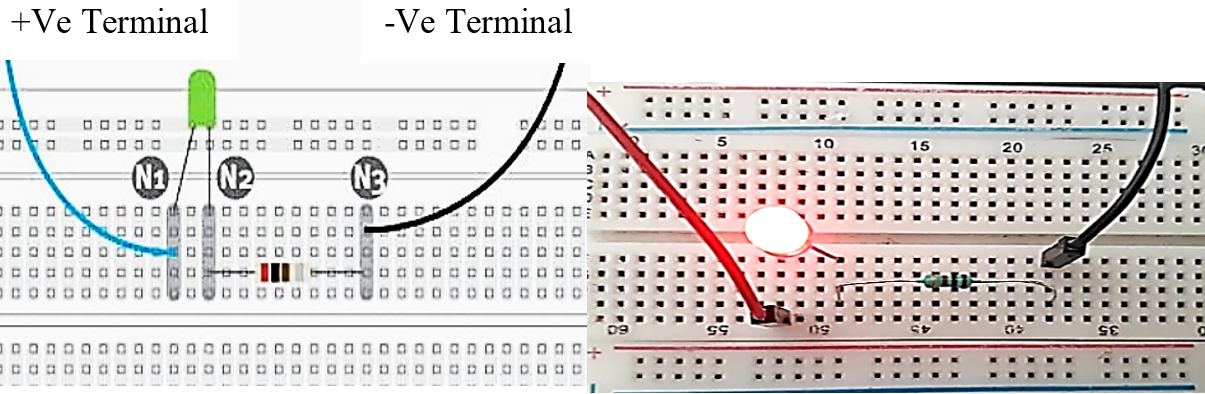
\includegraphics[scale=0.7]{EXP_26_I_Images/fig6.png}
\end{center}
\vspace{-10mm}
\begin{center} {Figure 6.MQTT test client}\end{center}

\begin{center} 
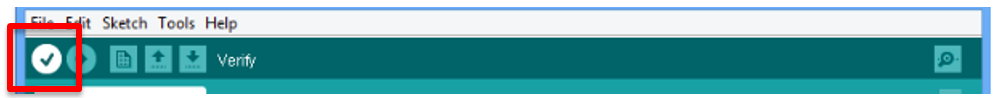
\includegraphics[scale=0.85]{EXP_26_I_Images/fig7.png}
\end{center}
\vspace{-10mm}
\begin{center} {Figure 7.The message is received on the MQTT test client}\end{center}

\end{itemize}

\noindent \textcolor{red}{Congratulations!} We have completed the most crucial part of the experiment. After testing is successful, disconnect the ESP32 from the PC/Laptop.\\[6pt]

\textbf{F) Storing the data from IoT devices to AWS DynamoDB}
\vspace{-3mm}
\begin{itemize}
 \setlength\itemsep{-0.3em}
\item Go to the AWS Console by clicking on the symbol \textbf{'aws'} in the top left corner. You can see the recently used AWS services.  Search \textbf{DynamoDB} on the search bar and click on it. Click on $ \rightarrow $ \textcolor{blue}{Create table} from the dashboard or click on $ \rightarrow $ \textcolor{blue}{Tables} and then $ \rightarrow $ \textcolor{blue}{Create table}.\par

A page as given in fig. 8 will appear. Put \textbf{Table name} as 'espdata'. In \textbf{Primary key}, we have to take that field from the payload which is unique and in our case it is \textbf{ID}, make it a \textbf{number}.We can add another field as a \textbf{sort key} for displaying the data in ascending/descending order based on that field. We leave it for time being. Then click on $ \rightarrow $ \textcolor{blue}{Create}.\par

A new page as given in fig.9  below will appear after clicking on \textcolor{blue}{Items}. Initially, it will be in the \textcolor{blue}{Overview} tab. Click on $ \rightarrow $ \textcolor{blue}{Create item}. A new page will open. Click on $ \rightarrow $ \textcolor{blue}{Tree. Text \& Tree} both options will appear. Select the $ \rightarrow $ \textcolor{blue}{Text}.



\begin{center} 
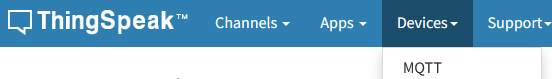
\includegraphics[scale=0.68]{EXP_26_I_Images/fig8.png}
\end{center}
\vspace{-10mm}
\begin{center} {Figure 8. DynamoDB table creation }\end{center}



Fill the JSON data structure as in our payload, a sample is given here, and click on$ \rightarrow $ \textbf{save}. This data will be stored in the espdata table and it can be seen in \textbf{items} of the table. We have done it for checking purposes only so we will delete this entry. For deleting, click on $ \rightarrow $ \textcolor{blue}{square box} in front of the ID and go to $ \rightarrow $ \textcolor{blue}{Actions} and  $ \rightarrow $ \textcolor{blue}{Delete}. 

\begin{center}
     Sample JSON data:\\[4pt]
\fbox{\begin{minipage}{6em}

\noindent \{\\
  "ID": 0, \\
  "temp":19,\\
  "humid":38\\
\}
\end{minipage}}
\end{center}

\begin{center} 
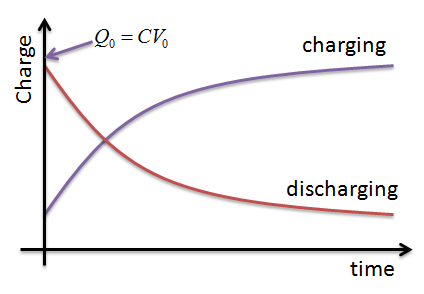
\includegraphics[scale=0.82]{EXP_26_I_Images/fig9.png}
\end{center}
\vspace{-10mm}
\begin{center} {Figure 9. DynamoDB table }\end{center}


\item \textbf{Rule Creation:} We have our table ready to accept the data from our IoT device. The next step is to create a rule. Again go to the $ \rightarrow $ \textcolor{blue}{AWS console} and go to the $ \rightarrow $ \textcolor{blue}{IoT core}, Click on $ \rightarrow $  \textcolor{blue}{Act} $ \rightarrow $  \textcolor{blue}{Rules}.
A new page will display, click on $ \rightarrow $ \textcolor{blue}{Create} a rule. Provide the rule \textbf{name} as \textbf{datastorerule} and in the \textbf{description}, we can write \textbf{'Rule for storing data'}.
\item In \textbf{Rule query statement write :  SELECT * FROM 'outTopic'}

The IoT device is publishing data on the topic- \textbf{"outTopic"} and we want all data to be stored in DynamoDB. Now Click on $ \rightarrow $  \textcolor{blue}{Add action}. A list of actions will be displayed as given in fig. 10 below.

\begin{center} 
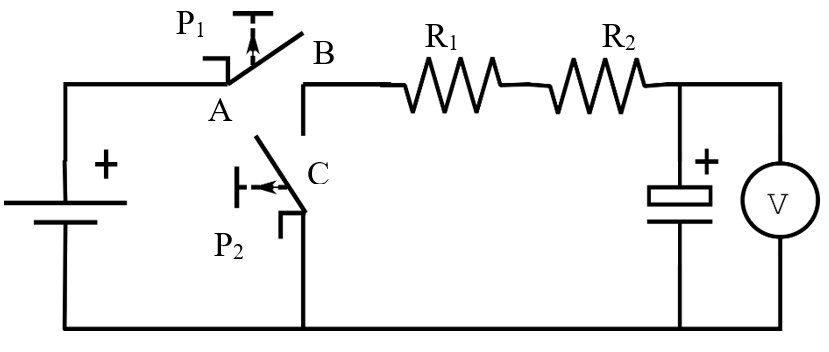
\includegraphics[scale=0.7]{EXP_26_I_Images/fig10.png}
\end{center}
\vspace{-10mm}
\begin{center} {Figure 10. Action list }\end{center}

Select the first one: \textbf{Insert a message into a DynamoDB table} and then click on $ \rightarrow $ \textcolor{blue}{Configure the action}. A new page as given in fig.11 below will appear. Click on $ \rightarrow $ \textcolor{blue}{Choose a resource} after refreshing it, select the table \textbf{'espdata'} that we had created in DynamoDB. In the \textbf{Partition key value} box, put the partition key field as it is coming from the IoT device in the payload. In our case it is \textbf{ID}. Keep dollar sign before ID (like $ \rightarrow $ \textbf{\$ID}). Click on $ \rightarrow $ \textcolor{blue}{Create Role}.\par
Provide the name of the role say \textbf{role4storage} and click on $ \rightarrow $ \textcolor{blue}{Create role}. Click on $ \rightarrow $ \textcolor{blue}{Add action}. Finally, click on $ \rightarrow $ \textcolor{blue}{create rule}. We can see the \textbf{datastorerule}, that we have created.

\begin{center} 
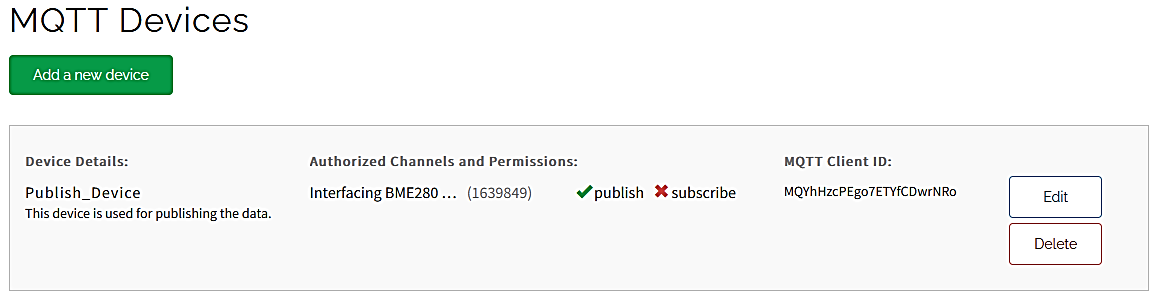
\includegraphics[scale=1]{EXP_26_I_Images/fig11.png}
\end{center}
\vspace{-10mm}
\begin{center} {Figure 11. Configure the action  }\end{center}

\item Connect the ESP32 and go to the DynamoDB . Check the table \textcolor{blue}{Items} after refreshing it. We can see the data being inserted in it as shown in fig.12 below. Click on $ \rightarrow $ the \textbf{square box} in front of \textbf{ID} and go to the $ \rightarrow $ \textcolor{blue}{Actions} from where we can export this data as a CSV file.

\begin{center} 
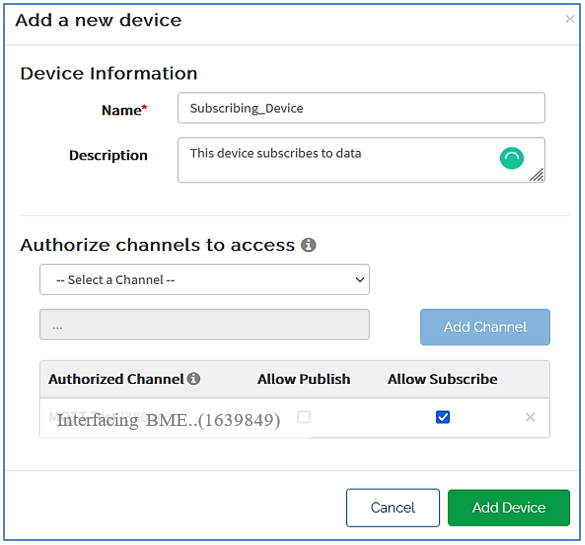
\includegraphics[scale=1]{EXP_26_I_Images/fig12.png}
\end{center}
\vspace{-10mm}
\begin{center} {Figure 12. Viewing data on the table  }\end{center}
\end{itemize}

\begin{center}
\textcolor{blue}{Congratulations!}\\
We have completed part-I of the experiment.
\end{center}

\noindent \textcolor{red}{Warning:} Don't keep the ESP32 powered on for a long duration. It publishes the data continuously and DyanamoDB free limit may cross.  It is advised to delete the table after completing the experiment. This will avoid data storage in case IoT device remains on unknowingly and AWS IoT core keep connected.

\vspace{10pt}
\noindent \textbf{\large REFERENCES:}
\vspace{-6mm}
\begin{enumerate}
\setlength\itemsep{-0.3em}

\item  \href {https://docs.aws.amazon.com/iot/latest/developerguide/iot-ddb-rule.html}{Storing device data in a DynamoDB table}

\item \href{https://aws.amazon.com/about-aws/whats-new/2018/02/aws-iot-core-now-supports-mqtt-connections-with-certificate-based-client-authentication-on-port-443/}{AWS IoT Core MQTT}

\item	\href {https://docs.aws.amazon.com/iot/latest/developerguide/example-iot-policies.html}{AWS IoT Core policy examples}

\item \href {https://docs.aws.amazon.com/IAM/latest/UserGuide/access_policies.html} {Policies and permissions in IAM}

\end{enumerate}


\noindent \textbf{\large CONCEPT DRILL}\\[6pt]
Integrate BME280 or any other sensor with ESP32 and publish the data to AWS-IoT and store it into a table in DynamoDB.

\end{justify}
\end{document}